\documentclass{article}
\usepackage{graphicx} % Required for inserting images
% --- Essential Math Packages -

% --- REQUIRED PACKAGES ---
\usepackage[utf8]{inputenc}
\usepackage{amsmath} % For math formatting
\usepackage{amssymb}
\usepackage{hyperref}

% TikZ and pgfplots are the core plotting packages
\usepackage{tikz}
\usepackage{pgfplots}

% Recommended setting for pgfplots compatibility
\pgfplotsset{compat=1.18}

% Define custom styles to make the code cleaner
\tikzset{
    dot/.style={circle, fill=blue, inner sep=1.5pt}, % Style for the dots
    dashed_line/.style={dashed, gray!80, thin},      % Style for dashed grid lines
    slope_arc/.style={->, bend angle=15, bend left, thin, blue!70} % Style for slope arrows
}


\usepackage{amsmath}   % Advanced math formatting
\usepackage{amssymb}   % Math symbols (like \mathbb{R})
\usepackage{amsthm}   % Theorem and proof environments
\usepackage{mathtools} % Useful tweaks for amsmath

% --- Language & Character Support ---
\usepackage[utf8]{inputenc} % Allows special characters
\usepackage[T1]{fontenc}    % Better font encoding
\usepackage[english]{babel} % Language support

% --- Layout ---
\usepackage[margin=1in]{geometry} % Standard 1-inch margins
\usepackage{parskip}              % Adds space between paragraphs (looks cleaner)







\title{ Convex Optimization - Exercises from Chapter 3 of Boyd}
\author{Constantinos Kontovrakis}
\date{March 2026}

\begin{document}

\maketitle

\section*{3.1}
\textbf{(a)}\noindent $f: \mathbb{R} \to \mathbb{R}$ convex, $a, b \in \textbf{dom } f$ with $a < b$ \\

\noindent Show that: (a) $f(x) \leq \left( \frac{b-x}{b-a} \right) f(a) + \left( \frac{x-a}{b-a} \right) f(b)$ \\

\noindent $f$ convex. \\
By Jensen's inequality :
$f(\theta x + (1-\theta)y) \leq \theta f(x) + (1-\theta) f(y)$ \\
For any $x$ in $[a, b]$ \\

\[ C_1 + C_2 = \frac{b-x}{b-a} + \frac{x-a}{b-a} = 1 \]

\noindent Applying Jensen's inequality: \\
$f(C_1 \cdot a + C_2 \cdot b) \leq C_1 \cdot f(a) + C_2 \cdot f(b)$ \\

\begin{align*}
C_1 \cdot a + C_2 \cdot b &= \frac{b-x}{b-a} \cdot a + \frac{x-a}{b-a} \cdot b \\
&= \frac{ab - ax + bx - ab}{b-a} \\
&= \frac{b-a}{b-a} \cdot x = x
\end{align*}

\[ f(x) = f(C_1 \cdot a + C_2 \cdot b) \leq C_1 \cdot f(a) + C_2 \cdot f(b) \]












\textbf{(b)} \noindent $\frac{f(x) - f(a)}{x - a} \leq \frac{f(b) - f(a)}{b - a} \implies$ \\

\noindent $f(x) - f(a) \leq \frac{x - a}{b - a} f(b) + \left( 1 - \frac{x - a}{b - a} \right) f(a) \implies$ \\

\noindent $f(x) \leq \underbrace{\left( \frac{x - a}{b - a} \right)}_{C_1} \cdot f(b) + \underbrace{\left( \frac{b - x}{b - a} \right)}_{C_2} f(a)$ \\

\noindent $C_1 + C_2 = \frac{x - a + b - x}{b - a} = 1$ \\


    Correct because $f(x)$ is convex

\noindent $\frac{f(b) - f(a)}{b - a} \leq \frac{f(b) - f(x)}{b - x} \implies -\frac{f(b) - f(x)}{b - x} \leq -\frac{f(b) - f(a)}{b - a} \implies$ \\

\noindent $\implies f(x) - f(b) \leq -\frac{b - x}{b - a} \cdot (f(b) - f(a)) \implies$ \\

\noindent $\implies f(x) \leq f(b) \cdot \left( 1 - \frac{b - x}{b - a} \right) + f(a) \cdot \frac{b - x}{b - a} \implies$ \\

\noindent $\implies f(x) \leq f(b) \cdot \underbrace{\left( \frac{x - a}{b - a} \right)}_{C_1} + f(a) \cdot \underbrace{\left( \frac{b - x}{b - a} \right)}_{C_2} \implies$ \\

\noindent \hspace*{2cm} With $C_1 + C_2 = 1$. Thus proved.




\begin{figure}[h]
    \centering
    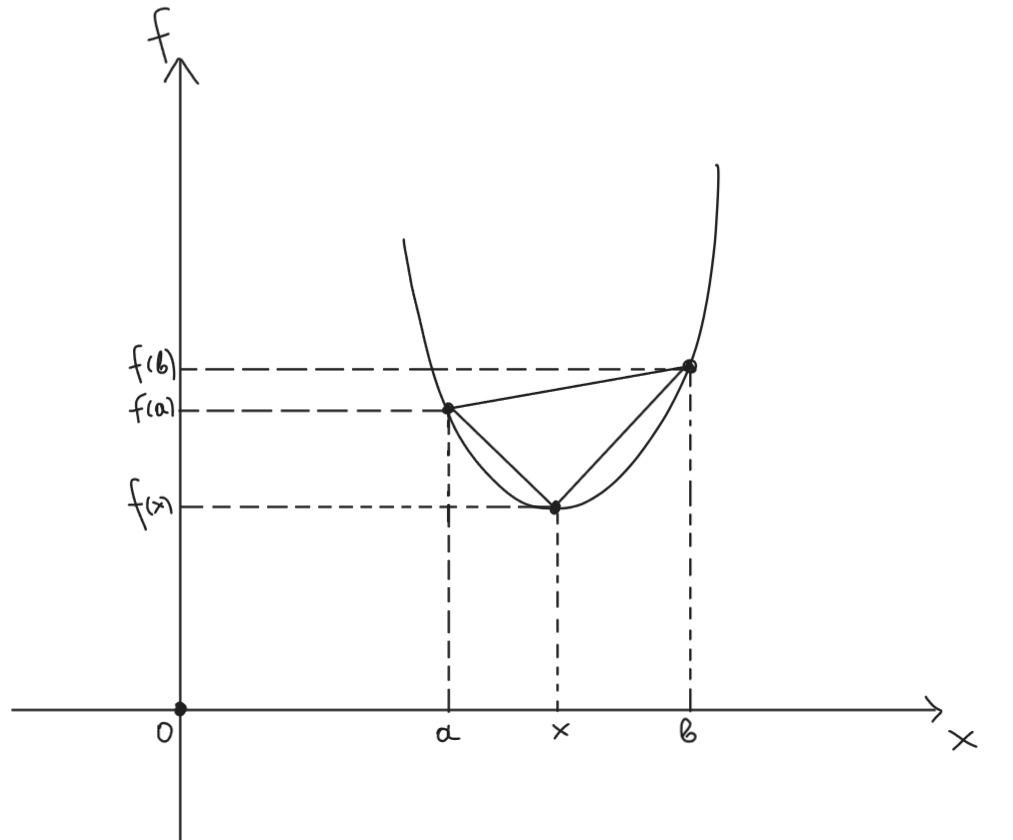
\includegraphics[width=1\linewidth]{slopess.png}
    \caption{Inequality of the slopes of intermediate point}
    \label{fig:placeholder}
\end{figure}






 \newpage
\textbf{(c)}For the left hand of the inequality:  \noindent $\forall x \in (a, b)$ \\

\noindent $\frac{f(x) - f(a)}{x - a} \leq \frac{f(b) - f(a)}{b - a} \implies$ \\

\noindent $\implies \frac{f(a + h) - f(a)}{a + h - a} \leq \frac{f(b) - f(a)}{b - a} \implies$ \\

\noindent $\implies \lim_{h \to 0^+} \frac{f(a + h) - f(a)}{h} \leq \frac{f(b) - f(a)}{b - a}$ \\

\noindent If $f$ differentiable, the limit exists and is equal to $f'(a) \implies f'(a) \leq \frac{f(b) - f(a)}{b - a}$


For the right hand of the inequality: 
\noindent $\forall x \in (a, b)$ \\

\noindent $\frac{f(b) - f(a)}{b - a} \leq \frac{f(b) - f(x)}{b - x} \implies$ \\

\noindent $\implies \frac{f(b) - f(a)}{b - a} \leq \frac{f(b) - f(b - h)}{b - (b - h)} = \frac{f(b) - f(b - h)}{h} \implies$ \\
\noindent replace $h \to -k$ \\

\noindent $\implies \frac{f(b) - f(a)}{b - a} \leq \frac{f(b + k) - f(b)}{k} \implies$ \\

\noindent $\implies \frac{f(b) - f(a)}{b - a} \leq \lim_{k \to 0^-} \frac{f(b + k) - f(b)}{k} \implies$ \\

\noindent $\implies \frac{f(b) - f(a)}{b - a} \leq f'(b)$














\textbf{(d)} \noindent Suppose that f is twice differentiable. Without loss of generality, we can write the previous inequality for any $a, b$. \\

\noindent For fixed $a$, and $h>0$ for $(a, a+h) \in \text{dom } f$ \\

\noindent $f'(a) \leq \frac{f(b) - f(a)}{b - a} \leq f'(b)$ \\
From monotonicity: \\ 
\noindent $f'(a) \leq \frac{f(a+h) - f(a)}{h} \leq f'(a+h) \implies$ \\

\noindent $\implies f'(a+h) - f'(a) \geq 0 \implies \frac{f'(a+h) - f'(a)}{h} \geq 0 \implies$ $   \lim_{h \to 0} \frac{f'(a+h) - f'(a)}{h} \geq 0   $\\

\noindent $\implies f''(a) \geq 0$



\noindent For fixed $b$, and $h > 0$ ,  for $(b-h, b) \in \text{dom } f$: \\ \noindent  $\frac{f(b) - f(a)}{b - a} \leq \frac{f(b) - f(b-h)}{h} \leq f'(b)$. \\ \noindent Replacing $h = -k$ : \\ \noindent $\implies \frac{f(b+k) - f(b)}{k} \leq f'(b) \implies \lim_{k \to 0^-} \frac{f(b+k) - f(b)}{k} \leq f'(b)$. \\ \noindent Since $b+k < b$ for $k < 0$, the monotonicity of the gradient implies $f'(b+k) \leq f'(b)$. \\ \noindent $\implies f'(b) - f'(b+k) \geq 0 \implies \frac{f'(b+k) - f'(b)}{k} \geq 0 \quad (\text{since } k < 0)$. \\ \noindent $\implies f''(b) = \lim_{k \to 0^-} \frac{f'(b+k) - f'(b)}{k} \geq 0$.

































\newpage
\section*{3.3}
\noindent For $x_1 < x_2 \implies f(x_1) < f(x_2)$ \\
For $y_1 < y_2 \implies g(y_1) < g(y_2)$ \\
\hspace*{2cm} $g$ is increasing \quad $\circledast$ \\

\noindent Let $x_1 = g(y_1)$, $x_2 = g(y_2)$ \\
\hspace*{0.5cm} $f(x_1) = y_1$, $f(x_2) = y_2$ \\

\noindent Combine: $x_\theta = \theta x_1 + (1-\theta) x_2$, \quad $\theta \in [0, 1]$ \\

\noindent $f \text{ convex} \implies f(x_\theta) \leq \theta f(x_1) + (1-\theta) f(x_2) \implies$ \\

\noindent $\xRightarrow{\circledast} g(f(x_\theta)) \leq g(\theta y_1 + (1-\theta) y_2) \implies$ \\

\noindent $\implies \theta x_1 + (1-\theta) x_2 = \theta \cdot g(y_1) + (1-\theta) g(y_2) \leq g(\theta y_1 + (1-\theta) y_2)$ \\

\noindent Thus $g$ is concave.


























\newpage
\section*{3.6}

\textbf{(a)}\noindent Let $y \in \mathbb{R}^{n+1} \implies y = (x, x_{n+1})$ with $x \in \mathbb{R}^n, x_{n+1} \in \mathbb{R}$ \\

\noindent Halfspace: for $\alpha \neq 0$
\[ H = \left\{ (x, x_{n+1}) \mid \alpha^T y \leq b, \alpha \in \mathbb{R}^{n+1}, b \in \mathbb{R} \right\} \]

\noindent for $\alpha^T = [ \alpha' \quad \alpha_{n+1} ]$ with $\alpha' \in \mathbb{R}^n, \alpha_{n+1} \in \mathbb{R}$ \\

\noindent $H \equiv \left\{ (x, x_{n+1}) \mid \alpha' x + \alpha_{n+1} x_{n+1} \leq b \right\}$ \\

\noindent $H \equiv \left\{ (x, x_{n+1}) \mid \alpha_{n+1} x_{n+1} \leq b - \alpha' x \right\}$ \\

For $a \neq 0$ :

\noindent For positive $\alpha_{n+1} \to H \equiv \left\{ (x, x_{n+1}) \mid x_{n+1} \leq \frac{b - \alpha' x}{\alpha_{n+1}} \right\}$ \\

\noindent For negative $\alpha_{n+1} \to H \equiv \left\{ (x, x_{n+1}) \mid x_{n+1} \geq \frac{b - \alpha' x}{\alpha_{n+1}} \right\}$ \\

\noindent In both cases $H$ is a halfspace, and we can define $f(x) = \frac{b}{\alpha_{n+1}} - \frac{\alpha'}{\alpha_{n+1}}x$ which is an affine function.

For the set to be equivalent to an epigraph of a function, we must choose only strictly negative $a_{n+1}$.

In conclusion for an epigraph of a function to be a halfspace, the function must be affine.

\textbf{(b)} \noindent $epi f = \text{cone}$ \\

\noindent $epi f = \left\{ (x, t) \mid x \in \mathbb{R}^n, t \geq f(x) \right\}$ \\

\noindent Cone: $\forall \ x \in C \implies \theta \cdot x \in C$ for $\theta \geq 0$ \\

\noindent $\theta \cdot (x, t) =  (\theta x, \theta t) \in C$ \\

\noindent For $epi f = \text{cone}$: \\

\noindent for $t \geq f(x) \implies \theta t \geq f(\theta x)$


On the boundary $t = f(x) \implies$
$    \theta \cdot f(x) \geq f(\theta x) \quad \text{ (1)}
$

\noindent For $x' = \theta x$, $\theta \cdot f(x) \geq f(x')$. \\
And from the cone property at the boundary of $epi f$:
\begin{align*}
    \frac{1}{\theta} \cdot f(x') &\geq f\left(\frac{1}{\theta} x'\right) \implies \\
    \frac{1}{\theta} f(\theta x) &\geq f(x) \implies \\
    f(\theta x) &\geq \theta f(x) \quad \text{ (2)}
\end{align*}
\noindent From (1), (2):
\begin{equation*}
    \left.
    \begin{aligned}
    \theta f(x) &\geq f(\theta x) \\
    f(\theta x) &\geq \theta f(x)
    \end{aligned}
    \right\} \implies \theta f(x) = f(\theta x) \quad \circledast
\end{equation*}

\noindent For $epi f$ to be a convex cone, the convex property must be satisfied:
\begin{equation*}
    f(\theta x_1 + (1-\theta)x_2) \leq \theta f(x_1) + (1-\theta) f(x_2) \quad \circledast\circledast
\end{equation*}
\noindent for $x_1, x_2 \in C$.

\noindent Thus the $epi f$ is a convex cone iff:
\begin{center}
    $\theta f(x) = f(\theta x)$ \\
    and \\
    $f(\theta x_1 + (1-\theta)x_2) \leq \theta f(x_1) + (1-\theta) f(x_2)$
\end{center}




\textbf{(c)}  \noindent $epi f = \text{polyhedron}$ \\

\noindent A polyhedron is an intersection of a finite number $m$ of constraints and inequalities.
\[ P = \bigcap_{i=1}^{m} \left\{ a^{i^T} x \leq b, \ C x = d  ,  x\in \mathbb{R}^{n+1}\right\}  \]

\noindent $epi f = \left\{ (x, t) \mid x \in \text{dom } f \subseteq\mathbb{R}^n  , \ t \geq f(x) \right\}$ \\

\noindent Let $a^{i} = \begin{bmatrix} a \\  a_{n+1} \end{bmatrix}$ \\

\noindent $a \cdot x + a_{n+1} \cdot x_{n+1} \leq b   \implies$ \\

\noindent $a_{n+1} \cdot x_{n+1} \leq b - ax$ \\

\noindent $\bullet$ $x_{n+1} \leq \frac{b - ax}{a_{n+1}}, \quad a_{n+1} > 0$ \\

\noindent $\bullet$ $x_{n+1} \geq \frac{b - ax}{a_{n+1}}, \quad a_{n+1} < 0$ \\

\noindent In this case with $a_{n+1} = 0$, the domain of f does not include $x_{n+1}$ .

\noindent We discard the first inequality, because the epigraph is unbounded from above.

\noindent We write the $i$-th inequality as:
\[ x_{n+1} \geq \frac{b - ax}{a_{n+1}} = \frac{b}{a_{n+1}} - \frac{a}{a_{n+1}} x \]

\noindent which is an affine function
\[ f_i(x) = \frac{b}{a_{n+1}} - \frac{a}{a_{n+1}} x \]

\noindent $x_{n+1} \geq f_i(x)$ \\
$t \geq f_i(x)$ \\

\noindent For $i = 1, \dots, m$ we get $m$ inequalities that must hold:
\[ t \geq f_1(x), \quad t \geq f_2(x), \dots, \quad t \geq f_m(x) \]

\noindent For all inequalities to hold simultaneously,:
\[ t \geq \max \{ f_1(x), \dots, f_m(x) \} \]









\newpage

\section*{3.7}

\noindent Suppose $f \neq c$ \\
$\exists \ x, y : f(x) < f(y) \iff f(y) - f(x) > 0$ \\

\noindent Let $z(t) = (1-t)x + ty$, for $t > 1$ \\
$ \ z \in \text{dom } f$, because $\text{dom } f = \mathbb{R}^n$ \\

\noindent We can write:
\[ y = \left( 1 - \frac{1}{t} \right)x + \frac{1}{t} z(t) \]

\noindent By convexity of $f$:
\[ f(y) \leq \left( 1 - \frac{1}{t} \right) f(x) + \frac{1}{t} f(z(t)) \implies \]

\noindent $\implies f(z(t)) \geq t \cdot f(y) - (t - 1) f(x) = f(x) + t \underbrace{(f(y) - f(x))}_{> 0}$ \\

\noindent We can arbitrarily choose $t$, which gives: \\

\noindent For $t \to \infty \implies f(z(t)) \to \infty$. \\

\noindent This contradicts $f$ being bounded above. \\

\noindent Thus $f = c$.





















\newpage
\section*{3.16}


\noindent \textbf{(a)}$f(x) = e^x - 1$ on $\mathbb{R}$ \\

\noindent $h(x) = e^x$ is strictly convex. \\
$g(x) = -1$ is affine. \\
$f(x) = h(x) + g(x)$ is convex as a non-negative sum of convex functions. \\

\noindent $f(x)$ is quasiconvex because it is convex.

\noindent Since $f(x) = e^x$ is strictly monotonic, it is by definition both quasiconcave and quasiconvex.

\medskip


\noindent \textbf{(b)}  $f(x_1, x_2) = x_1 \cdot x_2$ on $\mathbb{R}_{++}^2$ \\

\noindent $\partial_{x_1} f = x_2$ \\
$\partial_{x_2} f = x_1$ \\
$\partial_{x_1 x_1} f = 0$ \\
$\partial_{x_2 x_2} f = 0$ \\
$\partial_{x_1 x_2} f = 1$ \\
$\partial_{x_2 x_1} f = 1$ \\

\noindent $\nabla^2 f = \begin{bmatrix} 0 & 1 \\ 1 & 0 \end{bmatrix} = \mathcal{H}$ \\

\noindent For Hessian to be semidefinite: \\
$x^T \mathcal{H} x \geq 0$ \\

\noindent $\begin{bmatrix} x & y \end{bmatrix} \begin{bmatrix} 0 & 1 \\ 1 & 0 \end{bmatrix} \begin{bmatrix} x \\ y \end{bmatrix} = \begin{bmatrix} y & x \end{bmatrix} \begin{bmatrix} x \\ y \end{bmatrix} = 2xy$ \\

\noindent For positive semidefiniteness, the inequality $2xy \geq 0$ must hold for any vector. Which it does not, i.e., for $x=1, y=-1$. \\

\noindent Thus $f$ is not convex. \\
With similar steps we can show it is not concave either.


**An unnecessarily long \textbf{\hyperref[sec:qproof]{proof}} at the end of the file.**

Conclusively, $f$ is not quasiconvex.
With exactly symmetric reasoning, we conclude that f is quasiconcave, by showing that -f , has convex sublevel sets. 







\medskip

\textbf{(c)} \noindent $f(x,y) = \frac{1}{xy}$ \\

\noindent $\nabla^2 f(x,y) = H =  \begin{bmatrix} \frac{2}{x^2y^2} \cdot \frac{y}{x} & \frac{1}{x^2y^2} \\ \frac{1}{x^2y^2} & \frac{2}{x^2y^2} \cdot \frac{x}{y} \end{bmatrix} \implies \det H = \frac{4}{x^4y^4} \cdot \frac{yx}{xy} - \frac{1}{x^4y^4} = \frac{1}{x^4y^4} \cdot 3 > 0$ \\

\vspace{0.5cm}

\noindent Thus $f$ is strictly convex, therefore quasiconvex. \\
Also, $f$ is not concave nor affine.

\noindent $f(x_1, x_2) = \frac{1}{x_1 x_2} \quad , \quad x_1, x_2 \in \mathbb{R}_{++}^2$ \\[1.5em]

\noindent $f(x, y) = \frac{1}{xy} \longrightarrow g = -f = -\frac{1}{xy}$ \\[1em]

\noindent $S_a(g) = \{ x, y \mid -\frac{1}{xy} \leq a \ , \ x, y \in \mathbb{R}_{++}^2 \}$ \\[1.5em]

\noindent $-\frac{1}{xy} \leq a \quad , \quad \text{with } x, y > 0$ \\[1em]

\noindent $\frac{1}{xy} \geq -a \implies$
\begin{cases}
\text{For } a > 0 : \frac{1}{-ax} \leq y \ . \text{ This can be defined by the epigraph of } h_1(x) = -\frac{1}{ax} \ , \text{ with } a > 0 \\[1.5em]
\text{For } a < 0 : \frac{1}{-ax} \geq y \implies \frac{1}{ax} \leq y \ . \text{ Let } u = -y \implies \text{epi } h_2(u) \text{. With } h_2 = \frac{1}{ax} = u \ , \text{ with } a < 0, x > 0.
\end{cases}

\vspace{2.5em}

\noindent Both subsets must be convex for convexity of  $S_a$. \\[1.5em]

\noindent $h_2(x) = \frac{1}{ax} \quad , \quad a < 0 \ , \ x > 0$ \\[1em]

\noindent Is this a convex function? \\
\indent Let $k = -a > 0$ \\
\indent $h_2(x) = -\frac{1}{kx}$ \\[0.5em]
\indent $\nabla^2 h_2 = -\frac{2}{kx^3} < 0$ \\[1em]

\noindent Thus $h_2$ is not convex. \\[0.5em]

\noindent This means that $f$ is not quasiconcave.








\textbf{(d)} \noindent $f(x,y) = \frac{x}{y}$ on $\mathbb{R}_{++}^2$ \\

\noindent $\partial_x f = \frac{1}{y}$ \\
$\partial_{xx} f = 0$ \\
$\partial_{xy} f = -\frac{1}{y^2}$ \\
$\partial_y f = -\frac{x}{y^2}$ \\
$\partial_{yx} f = -\frac{1}{y^2}$ \\
$\partial_{yy} f = \frac{2x}{y^3}$ \\

\noindent $\nabla^2 f = H = \begin{bmatrix} 0 & -\frac{1}{y^2} \\ -\frac{1}{y^2} & \frac{2x}{y^3} \end{bmatrix} \implies \det H = -\frac{1}{y^4}$ \\

\noindent The function is neither convex nor concave. \\

\noindent Sublevel sets $f$: \\
$S_\alpha = \{ (x,y) \mid f(x,y) \leq \alpha, \, (x,y) \in \text{dom } f \} \equiv \left\{ (x,y) \mid \frac{x}{y} \leq \alpha, \, (x,y) \in \text{dom } f \right\}$ \\

\noindent We check for convexity. \\
$S_\alpha \equiv \{ (x,y) \mid x \leq \alpha y \implies x - \alpha y \leq 0 \implies A(x,y) \leq 0, \, (x,y) \in \text{dom } f \}$ \\
$A := \begin{bmatrix} 1 & -\alpha \end{bmatrix}$ \\

\noindent The set is convex because it is a linear combination.
\noindent For quasiconcavity: $f' = -f = -\frac{x}{y} \implies S'_\alpha = \left\{ (x,y) \mid -\frac{x}{y} \leq \alpha, \, (x,y) \in \text{dom } f \right\} \equiv \left\{ (x,y) \mid Ax \geq 0, \, (x,y) \in \text{dom } f \right\}$ \\

\vspace{0.5cm}

\noindent Thus $f$ is quasiconcave because the sublevel sets of $-f$ are convex.

\medskip

\\


\textbf{(e)}


\noindent $f(x_1, x_2) = \frac{x_1^2}{x_2} \quad , \quad \mathbb{R} \times \mathbb{R}_{++}$ \\[1.5em]

\noindent Hessian: \\[0.5em]
\begin{minipage}{0.3\textwidth}
\begin{align*}
\partial_x f &= \frac{2x}{y} \\
\partial_{xx} f &= \frac{2}{y} \\
\partial_{xy} f &= -\frac{2x}{y^2} \\
\partial_y f &= -\frac{x^2}{y^2} \\
\partial_{yx} f &= -\frac{2x}{y^2} \\
\partial_{yy} f &= \frac{2x^2}{y^3}
\end{align*}
\end{minipage}
\begin{minipage}{0.6\textwidth}
$H = \begin{bmatrix} \frac{2}{y} & -\frac{2x}{y^2} \\ -\frac{2x}{y^2} & \frac{2x^2}{y^3} \end{bmatrix} = 2 \frac{x^2}{y^2} \begin{bmatrix} \frac{y}{x^2} & -\frac{1}{x} \\ -\frac{1}{x} & \frac{1}{y} \end{bmatrix}$
\end{minipage}

\vspace{2em}

\noindent $\det H = 4 \frac{x^4}{y^4} \cdot \left( \frac{1}{x^2} - \frac{1}{x^2} \right) \implies \det H = 0$ \\[1.5em]

\noindent Semidefinite \\[0.5em]
\begin{align*}
x^T H x &= \begin{bmatrix} u & v \end{bmatrix} \begin{bmatrix} \frac{2}{y} & -\frac{2x}{y^2} \\ -\frac{2x}{y^2} & \frac{2x^2}{y^3} \end{bmatrix} \begin{bmatrix} u \\ v \end{bmatrix} = 2 \begin{bmatrix} u & v \end{bmatrix} \begin{bmatrix} \frac{u}{y} - \frac{x}{y^2} v \\ -\frac{xu}{y^2} + \frac{x^2 v}{y^3} \end{bmatrix} = \\[1em]
&= 2 \left( \frac{u^2}{y} - \frac{x \cdot uv}{y^2} - \frac{x \cdot uv}{y^2} + \frac{x^2 v^2}{y^3} \right) = 2 \left( \frac{u^2}{y} - \frac{2uvx}{y^2} + \frac{x^2 v^2}{y^3} \right) = \\[1em]
&= \frac{2}{y^3} \left[ u^2 y^2 - 2uvxy + v^2 x^2 \right] = \\[1em]
&= \frac{2}{y^3} (uy - vx)^2 \geq 0
\end{align*}

\vspace{1em}
\noindent Thus $H$ is positive semidefinite.
We conclude that f is convex and quasiconvex ,  not concave or affine. 

\noindent For quasiconcavity : 


\noindent $f(x_1, x_2) = \frac{x_1^2}{x_2}$ \\[1.5em]

\noindent $g = -f = -\frac{x_1^2}{x_2}$ \\[1em]

\noindent $S_a(g) = \{ (x_1, x_2) \mid -\frac{x_1^2}{x_2} \leq a \ , \ (x_1, x_2) \in \text{dom } g \}$ \\[1em]
\indent $\equiv \{ (x_1, x_2) \mid \frac{x_1^2}{x_2} \geq -a \ , \ (x_1, x_2) \in \text{dom } g \}$ \\[1em]
\indent $\equiv \{ (x_1, x_2) \mid x_1^2 \geq -a x_2 \ , \ (x_1, x_2) \in \text{dom } g \}$ \\[2em]

\noindent $x_1^2 \geq -a x_2 \longrightarrow$
\begin{cases}
\text{For } a = 0 : \frac{x_1^2}{x_2} \geq 0 \implies \mathbb{R} \times \mathbb{R}_{++} \text{, Convex} \\[1.5em]
\text{For } a > 0 : x_1^2 \geq -ax_2 \implies x_2 \geq -\frac{x_1^2}{a} \text{. Let } h_1(x_1) = -\frac{x_1^2}{a} \ , \ a > 0, x_1 \in \mathbb{R}. \\
\quad \quad \quad \quad \text{This holds for every $x_1 , x_2$ in $dom  \ g$. Thus $epi h_1$ is a convex set and $h_1$ is convex.   }  \\[1.5em]
\text{For } a < 0 : x_1^2 \geq -ax_2 \implies x_1^2 \geq kx_2 \implies x_2 \leq \frac{x_1^2}{k} \text{, with } k > 0. \\
\quad \quad \quad \quad \text{Let } h_2(x_1) = \frac{x_1^2}{k} \text{. This is the hypograph of a convex function,} \\
\quad \quad \quad \quad \text{thus non-convex for } a < 0.
\end{cases}

\vspace{2em}

\noindent This means that $S_a$ of $g$ are not always convex. \\
\noindent Thus $f$ is not quasiconcave.


\textbf{(f)} 

\noindent $f(x, y) = x^\alpha y^{1-\alpha} \quad , \quad \alpha \in [0, 1] \ , \ (x, y) \in \mathbb{R}_{++}^2$ \\[1.5em]

\noindent Hessian: $\nabla^2 f$ \\[0.5em]
\begin{align*}
\partial_x f &= \alpha x^{\alpha-1} y^{1-\alpha} \\
\partial_{xx} f &= \alpha(\alpha-1) x^{\alpha-2} y^{1-\alpha} \\
\partial_{xy} f &= \alpha(1-\alpha) x^{\alpha-1} y^{-\alpha} \\
\partial_y f &= (1-\alpha) x^\alpha y^{-\alpha} \\
\partial_{yx} f &= (1-\alpha)\alpha x^{\alpha-1} y^{-\alpha} \\
\partial_{yy} f &= (1-\alpha)(-\alpha) x^\alpha y^{-(1+\alpha)}
\end{align*}

\vspace{1em}

\noindent $\nabla^2 f = H = \begin{bmatrix} 
\alpha(\alpha-1)x^{\alpha-2}y^{1-\alpha} & \alpha(1-\alpha)x^{\alpha-1}y^{-\alpha} \\
(1-\alpha)\alpha x^{\alpha-1}y^{-\alpha} & (1-\alpha)(-\alpha)x^\alpha y^{-(1+\alpha)} 
\end{bmatrix}$ \\[1.5em]

\noindent $\det H = (\alpha)(-\alpha)(1-\alpha)(\alpha-1) \cdot x^\alpha x^{\alpha-2} y^{1-\alpha} y^{-(1+\alpha)} - (\alpha \cdot \alpha \cdot (1-\alpha)(1-\alpha) \cdot x^{\alpha-1} x^{\alpha-1} y^{-\alpha} y^{-\alpha})$ \\[1em]
\indent $= \alpha^2 (\alpha-1)^2 \left[ (x^{\alpha-1})^2 (y^{-\alpha})^2 - (x^{\alpha-1})^2 (y^{-\alpha})^2 \right] = 0$







\newpage

Semidefinite check : 
\noindent $x^T H x = \begin{bmatrix} u & v \end{bmatrix} \begin{bmatrix} \alpha (\alpha-1) x^{\alpha-2} y^{1-\alpha} & \alpha(1-\alpha) x^{\alpha-1} y^{-\alpha} \\ (1-\alpha)\alpha x^{\alpha-1} y^{-\alpha} & (1-\alpha)(-\alpha) x^\alpha y^{-(1+\alpha)} \end{bmatrix} \begin{bmatrix} u \\ v \end{bmatrix}$ \\[1.5em]

\noindent $= \begin{bmatrix} u \cdot \alpha(\alpha-1) x^{\alpha-2} y^{1-\alpha} + v(1-\alpha) \cdot \alpha \cdot x^{\alpha-1} y^{-\alpha} & u \cdot \alpha(1-\alpha) \cdot x^{\alpha-1} y^{-\alpha} + v(1-\alpha)(-\alpha) \cdot x^\alpha y^{-(1+\alpha)} \end{bmatrix} \begin{bmatrix} u \\ v \end{bmatrix} =$ \\[1.5em]

\noindent $= u^2 \alpha(\alpha-1) x^{\alpha-2} y^{1-\alpha} + uv \alpha(1-\alpha) x^{\alpha-1} y^{-\alpha} + uv \alpha(1-\alpha) x^{\alpha-1} y^{-\alpha} + v^2 (1-\alpha)(-\alpha) x^\alpha y^{-(1+\alpha)} =$ \\[1.5em]

\noindent $= -(1-\alpha) \alpha \cdot u^2 \cdot x^{\alpha-2} y^{1-\alpha} + 2uv \cdot (1-\alpha)\alpha \cdot x^{\alpha-1} y^{-\alpha} - (1-\alpha)\alpha \cdot v^2 \cdot x^\alpha y^{-(1+\alpha)} =$ \\[1.5em]

\noindent $= -(1-\alpha) \alpha \left[ u^2 \cdot \frac{x^\alpha}{y^\alpha} \cdot \frac{y}{x^2} - 2uv \cdot \frac{x^\alpha}{y^\alpha} \cdot \frac{1}{x} + \frac{x^\alpha}{y^\alpha} \cdot \frac{1}{y} \cdot v^2 \right] =$ \\[1.5em]

\noindent $= -(1-\alpha) \alpha \frac{x^\alpha}{y^\alpha} \left[ u^2 \cdot \frac{y}{x^2} - 2uv \cdot \frac{1}{x} + \frac{v^2}{y} \right] =$ \\[1.5em]

\noindent $= -(1-\alpha) \alpha \frac{x^\alpha}{y^\alpha} \cdot y \left[ u^2 \cdot \frac{1}{x^2} - 2uv \frac{1}{xy} + \frac{v^2}{y^2} \right] =$ \\[1.5em]

\noindent $= -\alpha(1-\alpha) \frac{x^\alpha}{y^\alpha} y \left[ \frac{u}{x} - \frac{v}{y} \right]^2 \leq 0$

\vspace{2em}

\noindent Thus $H$ is negative semi-definite. \\
\noindent This means that $f$ is concave and quasiconcave.





















\medskip \newline
\noindent $S_b = \{ (x, y) \mid x^\alpha \cdot y^{1-\alpha} \leq b \ , \ x, y \in \text{dom } f \}$ \\[1.5em]

\noindent $x^\alpha \leq y^{\alpha-1} \cdot b$ \\[1em]

\noindent $\bullet \ \alpha = 0 \longrightarrow 1 \leq \frac{b}{y}$, only true for $b \geq y$. \\[1em]


\noindent $\bullet \ \alpha = 1 \longrightarrow x \leq b$, which is a halfspace. \\[1em]



\noindent $\bullet \ 0 < \alpha < 1 \longrightarrow x \leq \sqrt[\alpha]{b \cdot y^{-1}} \cdot y \quad , \quad b > 0$ \\[1.5em]

\noindent $ - x \geq -\sqrt[\alpha]{b \cdot y^{-1}} \cdot y \quad $
\noindent Let $u=-x$

\noindent $ u \geq -\sqrt[\alpha]{b \cdot y^{-1}} \cdot y \quad  , u<0$
\noindent This is the epigraph of $h(y) = -\sqrt[\alpha]{b \cdot y^{-1}} \cdot y$ \\[1em]
\indent \text{with } $h(y) = -c \cdot y^{1 - \frac{1}{\alpha}} \quad , \quad \alpha \in (0, 1)$ \\[1.5em]

\noindent Curvature of  $h$: \\
\indent Since $1 - \frac{1}{\alpha} < 0$, the function $y^{1 - \frac{1}{\alpha}}$ is convex. \\
\indent Thus, $h(y) = -(\text{convex function})$ is concave. \\[1.5em]

\noindent Conclusion: $S_b$ is the epigraph of a concave function. The epigraph of a concave function is not always convex. Therefore, $f$ is not quasiconvex.

\newpage

\section*{3.22}


\textbf{(a)} \noindent Let $v = \sum_{i=1}^{n} e^{y_i}$. Since exponentials are strictly positive, $v > 0$. \\
\noindent For the outer logarithm to be defined, we require $-\log(v) > 0 \implies \log(v) < 0 \implies v < 1$. \\
\noindent Thus, our required starting input is restricted to $v \in (0, 1)$. \\[1.5em]

\noindent  $h_1(v) = \log v \quad \rightarrow \quad 
\begin{array}{|c|} 
\hline (0, 1) \\ \hline \nearrow \\ \hline 
\end{array} \quad 
\begin{array}{l} 
\text{Restricted dom: } (0, 1) \\ 
\text{Range: } (-\infty, 0) 
\end{array}$ \\[1.5em]

\noindent $\xrightarrow{\hspace{2cm}} \quad h_2(v) = -\log v = -h_1(v)$. \\
\indent \text{The range is multiplied by } -1 \text{.} \\[1em]

\noindent $h_2(v) = -\log v \quad \rightarrow \quad 
\begin{array}{|c|} 
\hline (0, 1) \\ \hline \searrow \\ \hline 
\end{array} \quad 
\begin{array}{l} 
\text{dom: } (0, 1) \\ 
\text{Range: } (0, +\infty) 
\end{array}$ \\[2em]

\noindent $\xrightarrow{\hspace{2cm}} \quad \text{Next is the outer function: } f(v) = -\log(h_2(v))$. \\
\indent \text{Since } h_2(v) \text{ outputs exactly into } (0, +\infty) \text{, it matches} \\
\indent \text{the required domain of the outer logarithm.} \\[1em]

\noindent  f(v) = -\log(h_2) \quad \rightarrow \quad 
\begin{array}{|c|} 
\hline h_2 \in (0, +\infty) \\ \hline \searrow \\ \hline 
\end{array} \quad 
\begin{array}{l} 
\text{Range: } (-\infty, +\infty) 
\end{array}$


\noindent $-\log(-\log(\sum e^{y_i}))$ \\[1em]

\noindent $g = \log(\sum e^{y_i}) \quad \text{is \textbf{convex}}.$ \\[1em]

\noindent $h_1(x) = -x \quad \text{non-increasing, linear.}$ \\[1em]

\noindent $h_2 = h_1(g) = -\log(\sum e^{y_i}) \quad \text{is \textbf{concave}}.$ \\
\indent \textit{(Linear non-increasing function of a convex function is concave.)} \\[1em]

\noindent $h_3 = \log h_2 : \quad 
\begin{cases} 
\log \text{ is concave, non-decreasing} \\
h_2 \text{ is concave} 
\end{cases}$ \\
\noindent \text{Thus } $h_3$ \text{ is \textbf{concave}}. \\[1em]

\noindent $h_4 = -h_3 : \quad
\begin{cases}
h_3 \text{ is concave} \\
-x \text{ is non-increasing, linear}
\end{cases}$ \\
\noindent \text{Thus } $h_4$ \text{ is \textbf{convex}}.


\newpage

\textbf{(b)}
\noindent $-\sqrt{u\left(v - \frac{x^T x}{u}\right)} \ , \ h_1 = \frac{x^T x}{u} \ , \ h_1 \text{ is convex}$ \\

\noindent $-\sqrt{u(v - h_1)} \ , \ h_2 = -h_1 \quad 
\begin{cases} 
h_1 \text{ convex} \\ 
-x \text{ non-increasing, linear} 
\end{cases} 
\text{, thus } h_2 \text{ is concave}$ \\

\noindent $-\sqrt{u(v + h_2)} \ , \ h_3 = v + h_2 \quad 
\{ \text{non-negative weighted sum preserves concavity} \} \quad 
\text{thus } h_3 \text{ concave}$ \\

\noindent $-\sqrt{u \cdot h_3} \ , \ \text{given that } -\sqrt{x_1 x_2} \text{ is convex} \quad 
\begin{cases} 
\sqrt{\cdot} \text{ is non-decreasing} \\ 
-x \text{ is decreasing} \\ 
-\sqrt{\cdot} \text{ is decreasing} 
\end{cases}$ \\

\vspace{1em}

\noindent $\left[ -\sqrt{h_3 \cdot u} \right] \ , \ 
\begin{cases} 
u \text{ linear (concave)} \\ 
h_3 \text{ concave} 
\end{cases} \ , \ -\sqrt{x_1 x_2} \text{ is non-increasing and convex.}$ \\

\vspace{1em}

\noindent From vector composition rules $f$  is convex.


\textbf{(c)} \noindent $-\log(uv - x^Tx)$ \\[1.5em]

\noindent $-\log((v - \frac{x^Tx}{u})u) = \underbrace{-\log u}_{h_1} - \underbrace{\log(v - \frac{x^Tx}{u})}_{h_2} \qquad \frac{x^Tx}{u} : \text{convex}$ \\[2em]

\noindent \textbf{Analysis of Component } $h_1$: \\
\indent $\log x : \text{concave}$ \\
\indent $-x : \text{linear, non-increasing}$ \\
\indent $h_1 : \text{convex}$ \\[1.5em]

\noindent \textbf{Analysis of Component } $h_3$: \\
\indent $\frac{x^Tx}{u} : \text{convex}$ \\
\indent $-x : \text{linear, non-increasing}$ \\
\indent $-\frac{x^Tx}{u} : \text{concave} \quad (h_3)$ \\[1.5em]

\noindent \textbf{Analysis of } $v + h_3$: \\
\indent $h_3 \text{ concave}$ \\
\indent $v : \text{linear and non-decreasing}$ \\
\indent $v + h_3 : \text{concave}$ \\
\indent (preservation on non negative sum) \\[1.5em]

\noindent \textbf{Analysis of Component } $h_2$: \\
\indent $v - \frac{x^Tx}{u} : \text{concave}$ \\
\indent $\log(x) : \text{concave, non-decreasing}$ \\
\indent $h_2 : \text{concave}$ \\[1.5em]

\noindent \textbf{Conversion of } $h_2$: \\
\indent $h_2 : \text{concave}$ \\
\indent $-x : \text{linear, non-increasing}$ \\
\indent $-h_2 : \text{convex}$ \\[1.5em]

\noindent \textbf{Final Combination:} \\
\indent $h_1 : \text{convex}$ \\
\indent $h_2 : \text{convex}$ \\
\indent $h_1 + h_2 : \text{convex}$ \\
\indent (preservation on non negative sum) \\[2em]

\noindent \textbf{Thus $f$ is convex}




\textbf{(d)} \noindent $-\left(t^p - \|x\|_p^p\right)^{1/p} =$ \\[1.5em]

\noindent $= -\left( t^{p-1} \left( t - \underbrace{\frac{\|x\|_p^p}{t^{p-1}}}_{g(x,t)} \right) \right)^{1/p}$ \\[1.5em]

\noindent $= -(t)^{1 - \frac{1}{p}} \cdot (\underbrace{t - g(x,t)}_{h})^{1/p} = -(t)^{1 - \frac{1}{p}} \cdot (h)^{1/p}$ \\[2em]

\noindent \textbf{Definition of } $g$: \\
\indent $g(x,t) = \frac{\|x\|_p^p}{t^{p-1}}$ \\
\indent Because norm is always non-negative we can use the property for $g(x,t)$ in $\text{dom } f$. \\[1.5em]

\noindent \textbf{Curvature Analysis (Step 1):} \\
\indent $g : \text{convex}$ \\
\indent $-x : \text{linear, non-increasing}$ \\
\indent $-g : \text{convex}$ \\[1.5em]

\noindent \textbf{Curvature Analysis (Step 2):} \\
\indent $t : \text{linear}$ \\
\indent $-g : \text{convex}$ \\
\indent $t - g : \text{convex}$ \\
\indent $h : \text{convex}$ \\[1.5em]

\noindent \textbf{Final Composition Logic:} \\
\indent It is given that: $-(x)^{1/p} (y)^{1 - 1/p}$ is convex. \\
\indent Also non decreasing in each component. \\
\indent $h : \text{convex}$ \\
\indent $t : \text{linear (convex)}$ \\[2em]

\noindent \textbf{Thus $f$ is convex.}




\textbf{(e)} \noindent $-\log\left(t^{p-1} \left(t - \frac{\|x\|_p^p}{t^{p-1}}\right)\right)$ \\[1.5em]

\noindent $= -\log t^{p-1} - \log\left(t - \frac{\|x\|_p^p}{t^{p-1}}\right)$ \\[1.5em]

\noindent $= -(p-1) \log t - \log\left(t - \underbrace{\frac{\|x\|_p^p}{t^{p-1}}}_{h_1}\right)$ \\[2em]

\noindent \textbf{Curvature Analysis (Step 1):} \\
\indent $h_1 : \text{convex}$ \\
\indent $-x : \text{linear, non-increasing}$ \\
\indent $-h_1 : \text{concave}$ \\[1.5em]

\noindent \textbf{Curvature Analysis (Step 2):} \\
\indent $t : \text{linear (concave)}$ \\
\indent $-h_1 : \text{concave}$ \\
\indent $t - h_1 : \text{concave}$ \\[1.5em]

\noindent \textbf{Composition Step 1:} \\
\indent $t - h_1 : \text{concave}$ \\
\indent $\log x : \text{concave, non-decreasing}$ \\
\indent $\log(t - h_1) : \text{concave}$ \\[1.5em]

\noindent \textbf{Composition Step 2:} \\
\indent $\log(t - h_1) : \text{concave}$ \\
\indent $-x : \text{linear, non-increasing}$ \\
\indent $-\log(t - h_1) : \text{convex}$ \\[1.5em]

\noindent \textbf{Final Conclusion:} \\
\indent $-\log t : \text{convex} \quad (\log x \text{ concave})$ \\
\indent $-\log(t - h_1) : \text{convex}$ \\
\indent Thus $-\log t - \log(t - h_1)$ \textbf{ Convex.}







\newpage
\section*{Extra 3.19}

\noindent $f, g : \mathbb{R}^n \to \mathbb{R}$ \\
$\phi : \mathbb{R} \to \mathbb{R}$ \\

\noindent \textbf{(a)} $f, g$ convex, then $h(x, y) = (f(x) + g(y))^2$ convex. FALSE \\


\noindent Let $u(x, y) = f(x) + g(y), \quad u : \mathbb{R}^n \to \mathbb{R}$ \\
\indent $u(x, y)$ is convex as a non-negative sum of convex functions. \\

\noindent Let $v(x) = x^2, \quad \mathbb{R} \to \mathbb{R}_+$ \\

\noindent We have $h(x, y) = v(u(x, y))$

\noindent v is convex and u is convex, 
\noindent but v is not non-decreasing.

\noindent (It would be convex if $f+g:  \mathbb{R}^n \to \mathbb{R}_+ $)

Counter-example : 
\noindent For $f(x)=x^2 $ and $g(y)=-1$ :  $v(f(x)+g(y)) = (x^2 - 1)^2$ \\
2nd order condition: \\
$\nabla^2 \left( (x^2 - 1)^2 \right) \geq 0 \implies$ \\

\noindent $\frac{\partial}{\partial x} \left( 2(x^2 - 1) \cdot 2x \right) =$ \\

\noindent $4(x^2 - 1) + 4x \cdot 2x = $ \\

\noindent $12x^2 - 4 \geq 0 \implies x^2 \geq \frac{1}{3}$ \\

\noindent False for $x \in \left( -1/\sqrt{3}, 1/\sqrt{3} \right)$

\begin{figure}[h]
    \centering
    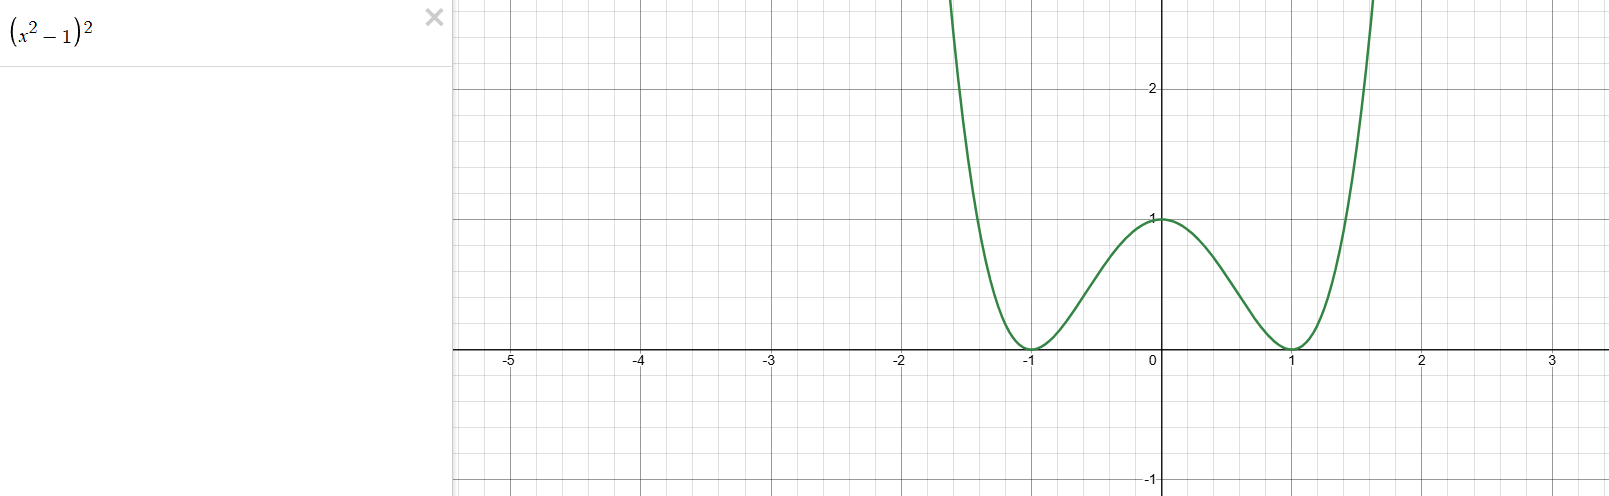
\includegraphics[width=1\linewidth]{image.png}
    \caption{Graphical representation of $f(x)=(x^2 - 1 )^2$}
    \label{fig:placeholder}
\end{figure}



\noindent \textbf{(b)} $f : \mathbb{R}^n \to \mathbb{R}$ \quad convex, differentiable \\
$\phi : \mathbb{R} \to \mathbb{R}$ \quad convex, differentiable \\
$\phi' > 0$ \\

\noindent Statement: $\phi(f(x))$ convex. TRUE\\

\noindent Check composition rule of differentiable convex functions: \\

\noindent $g = \phi(f(x))$ \\

\noindent $\phi$ convex and non-decreasing ($\phi' > 0$) \\
$f$ convex. \\

\noindent Thus $g$ is convex.




\textbf{(c)} \noindent From vector composition Rule: \\
\indent $u(x,y) = \sqrt{xy} , \quad u: \mathbb{R_{++}}^2 \to \mathbb{R}$: concave  (Geometric Mean) \\
\indent $f, g$: concave \\

\noindent $u(x,y)$ non-decreasing : 
$$ \frac{\partial u}{\partial x} = \frac{\partial}{\partial x} (xy)^{1/2} = \frac{1}{2}(xy)^{-1/2} \cdot y = \frac{y}{2\sqrt{xy}} = \frac{1}{2} \sqrt{\frac{y}{x}} $$\noindent Since $x > 0$ and $y > 0$, then $\frac{1}{2} \sqrt{\frac{y}{x}} > 0$. 
\noindent Similarly:$$ \frac{\partial u}{\partial y} = \frac{1}{2} \sqrt{\frac{x}{y}} > 0 $$\noindent  The function is non-decreasing in each argument.


\noindent $h(f(x), g(y)) = \sqrt{f(x) \cdot g(y)}$ \quad is concave.


\newpage

\section*{3.16(b) Proof for quasiconvexity/quasiconcavity}
\phantomsection
\label{sec:qproof}

\noindent $f(x_1, x_2) = x_1 \cdot x_2 \quad , \quad \text{dom}f = \mathbb{R}_{++}^2$ \\[1em]
\noindent Sublevel sets: $S_a = \{ (x_1, x_2) \mid x_1 \cdot x_2 \leq a \ , \ x_1, x_2 \in \text{dom}f \}$ \\[1em]
\noindent Let $(x_1, x_2)$ and $(x_1', x_2') \in S_a$ \\[0.5em]
\indent then: $\quad \theta \cdot (x_1, x_2) + (1-\theta)(x_1', x_2') \in S_a \quad \forall (x_1, x_2), (x_1', x_2')$ \\
\indent with $\theta \in [0,1]$ \\[0.5em]
\indent $(\theta x_1 + (1-\theta)x_1', \theta x_2 + (1-\theta)x_2') \in S_a$

\vspace{1em}

\begin{align*}
&\theta x_1 \cdot \theta x_2 + \theta x_1 \cdot (1-\theta)x_2' + (1-\theta)x_2 \cdot \theta x_1' + (1-\theta)^2 x_1' x_2' = \\[0.5em]
&\quad \theta^2 x_1 x_2 + x_1 x_2' \cdot (\theta - \theta^2) + (\theta - \theta^2)x_2 x_1' + (1-\theta)^2 x_1' x_2' = \\[0.5em]
&\quad \theta^2 x_1 x_2 - \theta^2 x_1 x_2' - \theta^2 x_2 x_1' + \theta^2 x_1' x_2' + x_1 x_2' \theta + \theta \cdot x_2 x_1' - 2\theta x_1' x_2' + x_1' x_2' = \\[0.5em]
&\quad \theta^2 (x_1 x_2 - x_1 x_2' - x_2 x_1' + x_1' x_2') + \theta \Big( \overbrace{x_1 x_2' + x_2 x_1' - 2x_1' x_2'}^{x_1 x_2' + x_2 x_1' - x_1' x_2' - x_1' x_2'} \Big) + x_1' x_2' = \\[0.5em]
&\quad \theta^2 \Big( x_1(x_2 - x_2') - x_1'(x_2 - x_2') \Big) + \theta \Big( x_1'(x_2 - x_2') + x_2'(x_1 - x_1') \Big) + x_1' x_2' = \\[0.5em]
&\quad \theta^2 \Big( (x_2 - x_2')(x_1 - x_1') \Big) + \theta \Big( x_1'(x_2 - x_2') + x_2'(x_1 - x_1') \Big) + x_1' x_2' \leq a
\end{align*}

\begin{align*}
&\frac{\theta^2 ((x_2 - x_2')(x_1 - x_1'))}{x_1' x_2'} + \theta \left( \left( \frac{x_2}{x_2'} - 1 \right) + \frac{x_1}{x_1'} - 1 \right) + 1 \leq \frac{a}{x_1' x_2'} \\[1em]
&\frac{\theta^2 ((x_2 - x_2')(x_1 - x_1'))}{x_1' x_2'} + \theta \left( \frac{x_2}{x_2'} + \frac{x_1}{x_1'} - 2 \right) + 1 \leq \frac{a}{x_1' x_2'}
\end{align*}

\vspace{1em}

\noindent $\left[ \text{By choosing points at the boundary : } x_1 x_2 = x_1' x_2' = a \implies \frac{x_1}{x_1'} = \frac{x_2'}{x_2} = 2c \right]$

\begin{align*}
&\frac{\theta^2((x_2 - x_2')(x_1 - x_1'))}{a} + \theta \left( \frac{1}{2c} + 2c - 2 \right) \leq 0 \\[1em]
&\theta^2 \frac{(x_2 - x_2')(x_1 - x_1')}{x_1' x_2'} + \theta \left( \frac{1}{2c} + 2c - 2 \right) \leq 0 \\[1em]
&\theta^2 \left( \frac{x_2}{x_2'} - 1 \right) \left( \frac{x_1}{x_1'} - 1 \right) + \theta \left( \frac{1}{2c} + 2c - 2 \right) \leq 0 \\[1em]
&\theta^2 \left( \frac{1}{2c} - 1 \right)(2c - 1) + \theta \left( \frac{1}{2c} + 2c - 2 \right) \leq 0 \\[1em]
&\theta^2 \left( 1 + 1 - \frac{1}{2c} - 2c \right) + \theta \left( \frac{1}{2c} + 2c - 2 \right) \leq 0 \\[1em]
&\theta^2 \left( 2 - \frac{1}{2c} - 2c \right) - \theta \left( 2 - \frac{1}{2c} - 2c \right) \leq 0 \\[1em]
&\theta^2 \cdot 2 \left( 1 - \frac{1}{4c} - c \right) - \theta \cdot 2 \left( 1 - \frac{1}{4c} - c \right) \leq 0
\end{align*}

\begin{align*}
&q := \left( 1 - \frac{1}{4c} - c \right) \\[0.5em]
&2 \cdot (\theta^2 \cdot q - \theta q) \leq 0 \\[0.5em]
&(\theta^2 - \theta) \cdot q \leq 0
\end{align*}

\vspace{1em}
\begin{align*}
q &= 1 - \frac{1}{4c} - c = \frac{c - \frac{1}{4} - c^2}{c} = -\frac{(c^2 - c + \frac{1}{4})}{c} = -\frac{(c - \frac{1}{2})^2}{c} < 0
\end{align*}

since $x_1, x_2, x_1', x_2' \in \mathbb{R}_{++}$, this is a negative expression $\left( \frac{x_1}{x_1'} = \frac{x_2'}{x_2} = c > 0 \right)$ and distinct points mean $c \neq \frac{1}{2}$. \\[1em]
Also because $\theta \in (0,1) \, , \, \theta^2 < \theta \implies \theta^2 - \theta < 0$ \\[1em]
Thus \quad $\underbrace{(\theta^2 - \theta)}_{(<0)} \cdot \underbrace{q}_{(<0)} \leq 0 \quad$ is a contradiction. \\[1em]
We supposed that the convex combination of any two points in the sublevel set \\
is in the sublevel set $S_a$ (convex set). 




















\end{document}

